\section{پردازش و موارد مطالعه داده‌های ‌چشمی و مغزی در اندازه گیری بارشناختی}
\label{s:data}
\subsection{صاف کردن و حذف نویز از داده‌های سیگنال مغزی}
در بخش
\ref{bbc:eeg_procon}
نویزهای مختلفی که می‌ تواند بر سیگنال دریافتی اثر بگذارد را دیدیم، گاهی این نویزها به قدری شبیه به امواج مغزی هستند که حتی افراد متخصص و با تجربه نیز نمی‌توانند به سادگی آن‌ها را از سیگنال اصلی تشخیص دهند. نویزها را می‌توان با توجه به عامل تولید کننده آن به دو دسته فیزیولوژیکی و غیر فیزیولوژیکی تقسیم کنیم. از جمله نویزهای فیزیولوژیکی که منشأ آن حرکات بدن است می‌توان به پلک زدن، حرکت سر، حرف زدن، بلعیدن و فعالیت الکتریکی قلب اشارده نمود، در دسته دیگر توزیع برق شهری، جابه‌جایی التکرودها بر روی سر و نویز تجهیزات ثبت سیگنال مثال‌هایی از غیر فیزیولوژیک هستند.
در شکل 
\ref{fig:eeg-blink-noise}
نمونه‌ای از نویز پلک زدن را مشاهده می‌کنید.
\begin{figure}[h]
	\centering
	\includegraphics[width=0.7\linewidth]{"figures/EEG blink noise"}
	\caption[نویز پلک زدن]{در قسمت‌های هاشور زده نمونه نویز پلک‌زدن مشخص شده‌است}
	\label{fig:eeg-blink-noise}
\end{figure}
جهت حذف نویز می‌توان ابتدا به صورت دستی فرکانس‌های بسیار بالا و پایین را حذف نمود و سپس از ابزار‌های آماده استفاده نمود. در فضای فرکانس با فیلتر بالا گذر
\LTRfootnote{High Pass Filter}
با فرکانس قطع ۰.۵ هرتز مي‌توان فرکانس نفس کشیدن را حذف نمود و برای اطمینان از حذف نویز برق شهری فرکانس ۵۰ هرتز با ناچ فیلتر
\LTRfootnote{Notch Filter}
حذف می‌شوند. از آن‌جا که الگوهای نویزهای یک دسته شبیه به هم هستند ابزار های هوشمندی چون جعبه ابزار کار با ای‌ای‌جی متلب به صورت خودکار آن‌ها را شناسایی کرده و حذف می‌کند.
\subsection{روش‌‌های استخراج ویژگی از داده‌های سیگنال مغزی}
ویژگی را می‌توان یک خصوصیت متمایز، اندازه‌گیری قابل تشخیص و یک مولفه کاربردی دانست که از بخشی از یک الگو بدست بیاید. به استخراج بخش‌های مهم اطلاعات و حذف  سایر قسمت‌های آن استخراج ویژگی  می‌گویند. برای به حداقل رساندن از بین رفتن اطلاعات مهم تعبیه شده در سیگنال، از استخراج ویژگی استفاده می‌شود. علاوه بر این، ویژگی‌ها میزان منابع مورد نیاز برای توصیف دقیق مجموعه عظیمی از داده ها را ساده‌تر می کنند. ویژگی‌ها برای به حداقل رساندن پیچیدگی های پیاده سازی برای کاهش هزینه پردازش اطلاعات و به منظور رفع نیاز احتمالی برای فشرده سازی اطلاعات استفاده می‌شوند.
\cite{al2014methods}
\\
اخیراً روش‌های متنوعی برای استخراج ویژگی‌ها از سیگنال‌های EEG به‌کار گرفته شده است، از میان آن‌ها می‌توان به این تبدیل‌ها اشاره نمود:
\begin{itemize}
	\item توزیع فرکانس زمان
	\LTRfootnote{time frequency distributions - TFD}
	\item تبدیل فوریه سریع
	\LTRfootnote{fast fourier transform - FFT}
	\item روش‌های مبتنی بر بردار ویژه
	\LTRfootnote{eigenvector methods - EM}
	\item تبدیل موجک گسسته
	\LTRfootnote{discrete wavelet transform - DWT }
	\item روش‌ خود همبسته
	\LTRfootnote{auto regressive method - ARM}
\end{itemize}
به جهت استفاده بیشتر از دو روش تبدیل فوریه سریع و تبدیل موجک گسسته در ادامه شرح این دو روش را خواهیم دید.
\subsubsection{تبدیل فوریه سریع}
\label{sssection:FFT}
سیگنال‌های EEG از شلیک یا اسپایک
\LTRfootnote{Spike}
همزمان نورون‌های عصبی شکل می‌گیرد و در طبیعت از فعالیت های دنبال شونده در طیف گسترده ای از فرکانس تشکیل شده است از این رو معمولا سیگنال‌های EEG را در فضای فرکانس تحلیل می‌کنند.
\cite{hu2019eeg}
در تبدیل فوریه، سیگنال مغزی که در حوزه زمان است را به حوزه فرکانس می‌بریم. این تبدیل مؤلفه‌های فرکانس ‌های موهومی یک سیگنال در حالت کلی نامتناوب را استخراج و نمایان می‌کند، در واقع تبدیل فوریه یک سیگنال، وزن فرکانس‌های موهومی موجود در سیگنال را نشان می‌دهد. به تبدیل فوریه یک سیگنال، طیف سیگنال
\LTRfootnote{Signal Spectrum}
 نیز گفته می‌شود.
 رابطه 
 \eqref{eq:DTFT}
 تبدیل فوریه سیگنال زمان گسسته
$  x_{n} $
 را نشان می‌دهد.
 \begin{equation}\label{eq:DTFT}
 X_{K}=\sum_{n=0}^{N-1}x_{n}e^{-i2\pi kn/N}
 \end{equation}
 که در آن N تعداد نمونه‌ها و n نمونه‌ فعلی است. $ x_{n} $ نشان دهنده مقدار سیگنال در زمان n و k  فرکانس فعلی (۰ هرتز تا N-1 هرتز) و $ X_{k} $ نتیجه حاصل از تبدیل فوریه گسسته است.
 محاسبه مستقیم تبدیل فوریه از رابطه
 \eqref{eq:DTFT}
 کند بوده و زمان زیادی می‌برد از این رو از الگوریتم تبدیل فوریه سریع که به صورت بازگشتی و با تقسیم و غلبه کار‌ می‌کند استفاده می‌کنند.
 شکل 
 \ref{fig:signal-analysis}
 به درک بهتر این تبدیل کمک می‌کند.
 \begin{figure}[h]
 	\centering
 	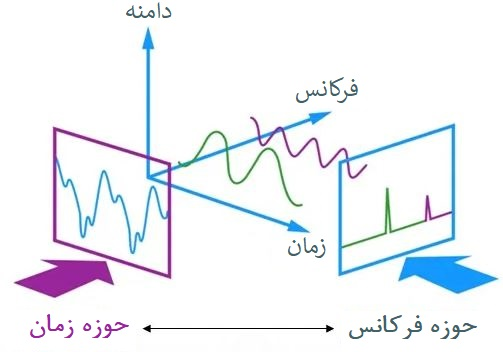
\includegraphics[width=0.7\linewidth]{figures/Signal-Analysis}
 	\caption[تبدیل فوریه]{تبدیل فوریه یک سیگنال دلخواه را از فضای زمان و یا مکان به فضای فرکانس می‌برد.\cite{fourier_transform}
 	}
 	\label{fig:signal-analysis}
 \end{figure}
 ولچ
 \LTRfootnote{Welch}
 یک روش بدون پارامتر تخمین همبستگی خودکار
 \LTRfootnote{autocorrelation}
 است. سیگنال‌های ثبت شده توسط تخمین چگالی توان (PSD)
 \LTRfootnote{power spectral density - PSD}
 محاسبه‌‌ می‌شوند. تا به صورت انتخابی نمایانگر نمونه‌های ای‌ای‌جی باشند.
\subsubsection{تبدیل موجک گسسته}
\label{sssection:DWT}
تبدیل فوریه تا زمانی که فرکانس‌های ظاهر شده در یک سیگنال وابسته به زمان نباشند به خوبی عمل خواهد کرد یا به عبارت دیگر اگر یک سیگنال شامل فرکانس x هرتز باشد، این فرکانس باید به صورت برابر در تمام طول سیگنال وجود داشته باشد.
دسته‌ی زیادی از سیگنال‌ها در طبیعت که فرکانس‌ ‌آن‌ها در طول زمان تغییر می‌کند را نا نمی‌توان با تبدیل فوریه با دقت و رزولوشن خوبی مدل کرد. از جمله این سیستم‌های دینامیک میتوان به داده‌های بازار بورس، بدن انسان و داده‌های برخی تجهیزات اشاره کرد. در این شرایط از تبدیل موجک که هم اطلاعات فرکانسی و هم اطلاعات زمانی را ذخیره می‌کند استفاده می‌کنیم.
\\
بنابراین در حالت کلی می‌توان گفت تبدیل موجک به صورت توافقی عمل می‌کند. در مقیاس‌هایی که مشخصه‌های وابسته به زمان مهم‌تر هستند، تبدیل موجک دارای دقت بالاتر در حوزه زمان و در مقیاس‌هایی که مشخصه‌های وابسته به فرکانس مهم‌تر هستند، دارای دقت بالاتر در حوزه فرکانس است. این نوع توافق دقیقا همان هدفی است که در پردازش سیگنال مورد نظر است.
\\
تبدیل موجک سیگنال یک بعدی ای‌ای‌جی، دارای دو بعد است. این خروجی دو بعدی مربوط به تبدیل موجک، نمایش سیگنال اصلی بر حسب مقیاس و زمان است که به طیف اسپکتروگرام 
\LTRfootnote{Spectrogram}
 یا اسکالوگرام
\LTRfootnote{Scaleogram}
معروف است. تبدیل موجک انواع متفاوتی دارد. برای انواع مختلف تبدیل موجک، مصالحه بین فشردگی 
\LTRfootnote{Compact}
 و صاف بودن 
\LTRfootnote{Smooth}
  با یکدیگر تفاوت دارند. به عبارت دیگر این خاصیت بیان می‌کند که می‌توانیم نوع خاصی از تبدیل موجک را انتخاب کنیم که با ویژگی مورد نظر برای استخراج از سیگنال تناسب بیشتری داشته باشد. یکی از انواع معرف آن هار
  \LTRfootnote{Haar}
  است.
  \\
روند کار در تبدیل موجک را در شکل 
  \ref{fig:wavelet-transform}
مشاهده می‌کنید.
در سطح صفرم ما یک سیگنال داریم و آن‌را در سطح اول به دو بخش تقریب
\LTRfootnote{Approximation}
 و جزئیات
\LTRfootnote{Detail}
  سیگنال تقسیم می‌کنیم. معمولا انتظار داریم نویز در بخش جزئیات باشد چون معمولا فرکانس نویز بالا است، تقریب اول شباهتش به سیگنال اصلی بیشتر است، از این رو می‌توان همان گونه که سیگنال اصلی را به دو بخش تجزیه کردیم تقریب اول را هم به دو بخش تقریب سطح دوم و جزئیات سطح دوم تجزیه می‌کنیم. این روند را تا جایی که جزئیات صفر و یا نزدیک به صفر شود انجام می‌دهیم . حال می‌توان سیگنال اصلی را با رابطه
  \eqref{eq:WaveletTransfrom}
  نشان داد. معمولا اگر به خواهیم نویزی را حذف کنیم از $ d_1 $ حذف می‌کنیم.
  
  \begin{equation}\label{eq:WaveletTransfrom}
  S = d_1 + d_2 + \cdots + d_N + a_N   
  \end{equation}
  اکنون به جای آنکه مستقیما سیگنال اصلی را به الگوریتم خود که می‌تواند شبکه عصبی، سیستم فازی یا شبکه بیزی
  \LTRfootnote{Bayesian network}
   باشد بدهیم، می‌تواینم ویژگی‌های استخراج شده یعنی $ d_1 $ تا $ d_N $ را بدهیم.
  \begin{figure}[h]
	\centering
	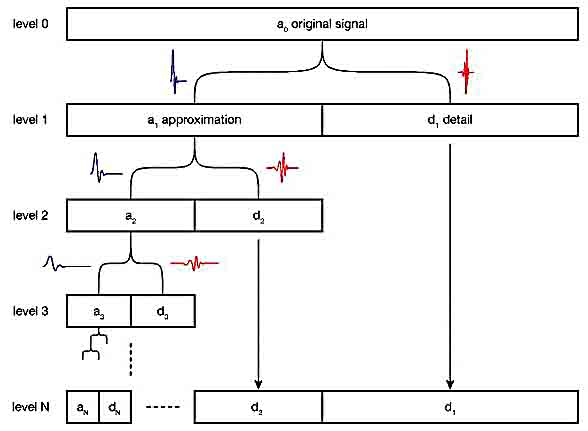
\includegraphics[width=\linewidth]{figures/wavelet-transform}
	\caption[تبدیل موجک]{بررسی اجمالی طرح تبدیل موجک گسسته، سیگنال اصلی به اجزای فرکانس پایین و فرکانس بالا تقسیم می شود ، که به ترتیب تقریب سیگنال و اطلاعات جزئیات را تشکیل می دهند. هر سطح اطلاعات تقریبی را بیشتر تجزیه می کند ، و هر سطح جزئیات یک باند فرکانس جداگانه را تشکیل می دهد\cite{sundling2006wavelets}}
	\label{fig:wavelet-transform}
\end{figure}

\subsubsection{مقایسه روش‌های استخراج ویژگی}
در دو زیر بخش
\ref{sssection:FFT}
و
\ref{sssection:DWT}
به ترتیب با تبدیل فوریه سریع و تبدیل موجک آشنا شدیم در این قسمت قصد داریم تا این دو تبدیل را با هم مقایسه و مزایا و معایب هریک را عنوان نماییم. استفاده مناسب از هر کدام می‌تواند راه حل خوبی باشد.
\\
در جدول
\ref{tab:FFT-VS-DWT}
می‌توانید مقایشه این دو روش را مشاده نمایید.

\begin{table}[]
	\caption[مقایسه تبدیل فوریه و موجک]{مقایسه مزایا و معایب دو روش تبدیل فوریه سریع و تبدیل موجک گسسته}
	\label{tab:FFT-VS-DWT}
	\begin{tabular}{ccc}
		\hline
		نام روش                                                        & مزیت‌ها                                                                                                                                                                                                 & معایب                                                                                                                                                                 \\ \hline
		\begin{tabular}[c]{@{}c@{}}تبدیل\\  فوریه\\  سریع\end{tabular} & \begin{tabular}[c]{@{}c@{}}-اغلب می‌تواند برای سیگنال‌های ایستا\\ (میانگین و واریانس در طول زمان ثابت باشد)\\  خوب عمل کند\\ -برای کارهای بلادرنگ \\ \\ تقریبا سریع تر از روش‌های دیگر است\end{tabular} & \begin{tabular}[c]{@{}c@{}}برای سیگنال‌هایی که فرکانس آن\\  در طول زمان تغییر کند مناسب نیست-\\ نمی‌تواند پیک‌های موجود را\\  با رزلوشن مناسبی  نشان دهد\end{tabular} \\ \hline
		\begin{tabular}[c]{@{}c@{}}تبدیل\\  موجک\end{tabular}          & \begin{tabular}[c]{@{}c@{}}اندازه پنجره آن متغییر است-\\ بین زمان و فرکانس مصالحه دارد-\\ -برای تجزیه و تحلیل سیگنال‌های\\  دارای تغییرات ناگهانی مناسب است\end{tabular}                                & -نیازمند انتخاب موجک مدار مناسب                                                                                                                                       \\ \hline
	\end{tabular}
\end{table}
\subsection{موارد مطالعه‌ی استفاده از داده‌های مغزی در سنجش بارشناختی}
در این زیر بخش به تعدادی پژوهش برجسته که در آن‌ها رابطه میان بارشناختی و سیگنال مغزی بررسی شده است خواهیم پرداخت. از میان آن‌ها نیز پژوهش‌هایی که به طور خاص با آزمایش‌ها و فعالیت‌هایی که محرک آن‌ها چند رسانه‌ای است در این مرور نقش مهم‌تری دارند.
\\
جِروْ و همکاران
\cite{gerve1999multimedia}
به بررسی بارشناختی حاصل یادگیری از چندرسانه‌ای از طریق سیگنال‌های مغزی پرداختند. در آزمایش آن‌ها که ۳۸ دانش آموزش مشارکت داشتند ۱۹ نفر مستعد و ۱۹ نفر معمولی. سه دسته محرک نمایش داده شد. متن؛ متن، تصویر و صدا؛ متن،‌صدا و فیلم و  در این حال امواج مغزی آن‌ها ثبت می‌شد. در طول نشان دادن متن مشاهده شد که توان باند آلفا بیشترین دامنه (فعالیت ذهنی کمتر) را در لوب‌های پس‌سری و گیج‌گاهی دارد و دامنه کم آن (فعالیت ذهنی بالاتر) در لوب پیشانی دیده شد. همچنین آن‌ها دیدند که دانش‌آموزان مستعد در هر سه محرک فعالیت ذهنی کمتری دارند.
\\
یزدانی و همکاران 
\cite{yazdani2009implicit}
به معرفی یک واسط رایانه مغز پرداختند که می‌تواند به صورت ضمنی محتوای‌ چندرسانه‌ای را از لحاظ احساسات مختلف برچسب بزند؛ به طوری که حتی داده‌های فردی که هنوز در آزمایش شرکت نکرده بود نیز به خوبی  قابل پیش‌بینی بود. در آزمایش آن‌ها نیز ۹ دانشجوی دکتری شرکت کرده بودند و از آن‌ها داده های سیگنال مغزی در حالی که چندرسانه‌ای را نگاه می‌کردند گرفته می‌شد.
\\
کاسترو و همکاران
\cite{castro2020validating}
به اعتبارسنجی باند تِتا به عنوان یک معیار عینی برای اندازه‌گیری بارشناختی در فیلم‌های آموزشی پرداختند. آن‌ها سه متن با سختی‌های متفاوت تولید کردند که یک راوی آن‌ها را می‌خواند. از شرکت کنندگان علاوه بر داده‌های مغزی و پرسشنامه فعلایت ذهنی، آزمون یادآوری نیز گرفته می‌شد. آن‌ها مشاهده کردند باند تتا و آزمون یادآوری برای ساده‌ترین و سخت ترین به خوبی می‌توانند تمیز دهنده این دو وضعیت باشند.
\\
آن‌ها فیلم‌های سخنرانی خود را به کمک دو معیار سطح بندی کردند. معیار اول سهولت خواندن
\LTRfootnote{reading ease}
بود. این معیار خوانایی متن را با شمارش تعداد هجا‌ها، کلمات و جملات انجام می‌دهد. خروجی آن یک عدد بین صفر تا صد است که هرچه بیشتر باشد نشان دهنده ساده‌تر و خوانایی بیشتر متن است. معیار دوم سهولت نحوی
\LTRfootnote{Syntactic simplicity}
بود. این معیار بر اساس چگالی عبارات اسمی، گروه معنایی کلمه‌ها و کلاس یک کلمه یک خروجی عددی می‌دهد که هرچه این عدد بزرگتر باشد نشان دهنده ساده‌تر بودن آن است. در آزمایش آن‌ها نیز ۳۵ نفر شرکت کرده بودند.
\\
آنتنکو و نایدرهاوسر
\cite{antonenko2010influence}
به بررسی بارشناختی حاصل از مطالعه متون حاوی هدایت‌گر از طریق سیگنال مغزی پرداختند. تفاوت میان متن معمولی و متن دارای هدایت‌گر در این است که در متن معمولی اگر خواننده به مفهومی برخورد کند که معنای آن را نداند باید از حافظه بلند مدت خود آن را به حافظ فعال فراخوانی و یادآوری کند از طرفی دیگر ساختمان و چینش مفاهیم دست نویسنده متن است. این در حالی است که در متن شامل هدایت‌گر خواننده هرگاه به مفهومی برخورد کند که معنای آن را نمی‌داند می‌تواند به عنوان مثال نشان‌گر موس را بر روی کلمه مورد نظر قرار دهد بعد از آن مفاهیم کلی مرتبط با آن برای مدت کوتاهی بر روی صحفه ظاهر می‌شوند.
\\
در آزمایش آن‌ها که ۲۰ نفر شرکت کرده بودند، و علاوه بر داده‌های مغزی رفتار آن‌ها با سیستم به وسیله یک نرم افزاری که از صحفه به صورت مداوم تصویر برداری می‌کرد نیز ذخیره شد. به دلیل آنکه توجه بر اثرات حضور و عدم حضر هدایت‌گر بود در حالت بدون هدایت گر ۱۰ ثانیه اول شروع کار متن بررسی و در حالتی که هدایت گر وجود داشت ۱۰ ثانیه نخست پس از مشاهده اولین هدایت گر بررسی شد. با مقایسه نتایج پرسشنامه‌ای که خود شرکت‌کنندگان در رابطه بار شناختی خود اظهار نظر می‌کردند و داده‌های مغزی دیده شد که افراد در پرسش‌نامه نتوانستند به خوبی بین متن شامل هدایت‌گر و بدون هدایت گر تمیز قائل شوند، در طرف مقابل داده‌های مغزی به وضحوح میان این دو حالت تفاوت قائل شده بود.
\\
دَن و همکاران
\cite{dan2017eeg}
با آزمایش بر روی ۱۷ نفر قصد داشتند تا صفحات نمایشگر دو بعدی مثل نمایشگر‌های کامپیوتر، موبایل و تلویزیون را با نمایشگر‌های سه بعدی در بارشناختی ایجاد شده از طریق اندازه‌گیری سیگنال‌های مغزی اندازه‌گیری کنند. فعالیت‌ آن‌ها کاغذ و تا بود. در یک مرحله ساخت یک اوریگامی را بر روی نمایشگر دو بعدی می دیدندو در مرحله دیگر دقیقا ساخت همان اوریگامی را اما این با یک پروژکتور سه بعدی نگاه می‌کردند. از میان باند‌های مغزی باند آلفا و تتا نیز ذخیره شد. در میان شرکت کنندگان افرادی که توانایی کمتری در استعدادی فضایی و مکانی داشتند از نمایشگر‌های سه بعدی منفعت بیشتری بردند.
\\
مظاهر و همکاران
\cite{mazher2017eeg}
قصد داشتند با استفاده از استخراج ویژگی و انسجام جزئی‌گرا
\LTRfootnote{Partial Directed Coherence - PDC}
بر روی داده‌های سیگنال مغزی برای آزمایش چندرسانه‌ای بارشناختی را اندازه‌گیری کنند. داده‌ها از ۳۴ شخص سالم با یک دستگاه الکتروانسفالوگرافی ۱۲۸ کاناله با نرخ فرکانس ۲۵۰ هرتز ذخیره کردند.  در قسمت اول آزمایش برای ثبت سیگنال پایه
\LTRfootnote{base line}
از شرکت‌کنندگان خواسته می‌شد تا چشم‌هایی خود را ببندند و در حالت آرامش باشند. در قسمت دوم آزمایش به آن‌ها ۳ فیلم که از پیش تهیه شده و در سه سطح سختی متفاوت بودند نمایش داده می‌شد. پس از آن در طی ۳۰ ثانیه از آن‌ها آزمون یادآوری و فراخوانی حافظه گرفته می‌شد.
\\
آن‌ها به دلیل ماهیت غیرایستا بودن سیگنال‌های مغزی بر خلاف اکثر پژوهش‌های گذشته که از تبدیل فوریه سریع استفاده می‌کردند از تبدیل موجک گسسته استفاده کرند. به منظور تجزیه و تحلیل اتصلات مغزی از انسجام جزئی گرا یا به اختصار PDC استفاده کردند.
\\
فرض کنید دو سیگنال(یا فرآیند تصادفی) X و Y داشته باشیم از هر کدام مشاهدات گسسته x(t) و y(t) موجود باشد و $ t = 1,2, \dots, N $. ارتباط توأمان این دو سیگنال می‌تواند توسط مدل‌های دو متغیره خودکاهشی 
\LTRfootnote{bivariate autoregressive - ARX}
توصیف شود.
\begin{equation}
\label{eq:ARX1}
x(t)=\sum_{k=1}^{q} a_{11, k} x(t-k)+\sum_{k=1}^{q} a_{12, k} y(t-k)+e_{x}(t)
\end{equation}
\begin{equation}
\label{eq:ARX2}
y(t)=\sum_{k=1}^{q} a_{21, k} x(t-k)+\sum_{k=1}^{q} a_{22, k} y(t-k)+e_{y}(t)
\end{equation}
مدل‌های خطی 
\eqref{eq:ARX1}
و
\eqref{eq:ARX2}
می‌توانند با تبدیل فوریه به صورت ماتریسی و در حوزه فرکانس نوشته شوند.
\begin{equation}
\label{eq:PDC1}
\left(\begin{array}{ll}
A_{11}(f) & A_{12}(f) \\
A_{21}(f) & A_{22}(f)
\end{array}\right)\left(\begin{array}{l}
X(f) \\
Y(f)
\end{array}\right)=\left(\begin{array}{l}
E_{x}(f) \\
E_{y}(f)
\end{array}\right)
\end{equation}
\begin{equation}
\label{eq:PDC2}
\pi_{X \rightarrow Y}(f)=\sum_{k=1}^{q} a_{21, k} x(t-k) \frac{A_{21}(f)}{\sqrt{\left|A_{11}(f)\right|^{2}+\left|A_{21}(f)\right|^{2}}}
\end{equation}
$ \pi_{X \rightarrow Y} $
قدرت اتصال نسبی تعامل از یک منبع سیگنال مانند X به یک سیگنال دیگر مانند Y را توصیف می کند؛ در مقایسه (یا نرمال شده) با تمام اتصالات منبع به سیگنالهای دیگر. برای یک سیستم دو متغیره یک تعامل یک طرفه به صورت $ A_{21} $ نشان داده شده و نرمال سازی شده توسط عبارات مربوط به x در مدل ARX مثل $ A_{11} $ و $ A_{21} $. مقدار PDC بین صفر و یک خواهد بود. در نهایت آن‌ها میان امواج آلفا و بار شناختی از طریق قوانینی که بیان کرده بودند رابطه یپدا کردند.
\subsection{موارد مطالعه‌ی استفاده از داده‌های چشمی در سنجش بار شناختی}
دارِل رادمن و همکاران
\cite{Rudmann2003}
با نشان دادن تصویر چند چرخ‌دنده متصل بهم در تعداد و حالت‌ها مختلف از شرکت کنندگان می‌خواستند تا جهت چرخش هر یک از آنها را مشخص کند و با ذخیره داده های چشمی شرکت کنندگان به بررسی رابطه میان داده های چشمی و بار شناختی پرداختند. مطالعه‌های آنها نشان داده است که ، در یک کار ساده ، رفتار چشم تمایل دارد دنباله مورد انتظار از یک مدل مبتنی بر تحلیل وظیفه شناختی را دنبال کند. حال تحلیل و دسته بندی زمان هایی که کاربران این دنباله را متوقف کرده و به جای دیگر نگاه می‌کنند می‌تواند، وضعیت شناختی افراد را بیان نماید. در این بررسی آنها رابطه ای پیدا نکردند شاید به دلیل اینکه آزمایش دهندگان به خوبی با شرایط آزمایش خو نگرفته و آموزش ندیده بودند.
\\
در تجربه دوم که به بررسی این فرضیه می‌پرداخت که شرکت کنندگان به چیزی فکر می‌کنند که به آن نگاه می‌کنند، در این آزمایش در میانه تصویر صحفه را قطع می‌کردند و از آنها می‌خواستند تا به هرچه فکر می کنند را اعلام نمایند. نشان داده شد در اکثر موارد هرگاه کاربران به شیئی در تصویر خیره می‌شوند همان را گزارش می‌دهند.
\\
در کار دیگری مانوئل گارسیا باروس و همکاران،
\cite{Garcia-Barrios2004}
به ارائه‌ی چارچوبی برای یادگیری الکترونیکی با ردیاب چشمی پرداختند. آنها با چهار معیار تعداد و سرعت پرش چشمی و تعداد و مدت زمان تثبیت چشم مدلی انطباقی برای یادگیری الکترونیکی معرفی کردند، این مدل که در سمت معلم به کتابخانه‌ای از اطلاعات و محتواها متصل بود، با توجه به سطح بار شناختی یادگیرنده متحوای مناسب را تهیه می‌کند،‌از این رو یادگیری اثربخش تری برای یادگیرنده رخ می‌دهد.
\\
کِهارا و کروسبی
\cite{Ikehara2005}
با داده گرفتن از ۱۳ دانشجوی بین ۱۸ تا ۲۱ سال نیروی هوایی آمریکا به بررسی داده های چشمی پرداختند.
آنها کسرهای متحرک یا به اختصار MTF
\LTRfootnote{Moving Trgets Fractions}
را بررسی کردند. در این آزمایش تعداد ثابتی بیضی در صحفه نمایش داده می‌شود که شامل یک کسر است. این بیضی به صورت تصادفی در قسمتی از چپ تصویر نمایش داده می‌شوند و پس از مدتی به سمت راست صحفه منتقل می‌شوند. و از کاربر خواسته می‌شود تا آنهایی را که بیش از ۱/۳ هستند را پیش از آنکه به راست صحفه منتقل شود، مشخص کند.
\\
مشاهده شد که میان سختی آزمایش و داده های چشمی ارتباط وجود دارد و داده های چشمی به وضوح می‌تواند سطح سختی آزمایش را مشخص کند آنها به طور خاص زمان تثبیت و میزان حرکت چشم در بازه های زمانی را معیار گرفته بودند. همچنین بیان کردند که هنگامی که اجزا موجود در تصویر حرکت می‌کنند و مکانشان نامشخص است اندازه گیری نیز پیچیده می‌شود.
در شکل 
\ref{fig:ikehara2005}
سیستم آزمایش آنها نمایش داده شده است.
\\
\begin{figure}[htbp]
	\centering
	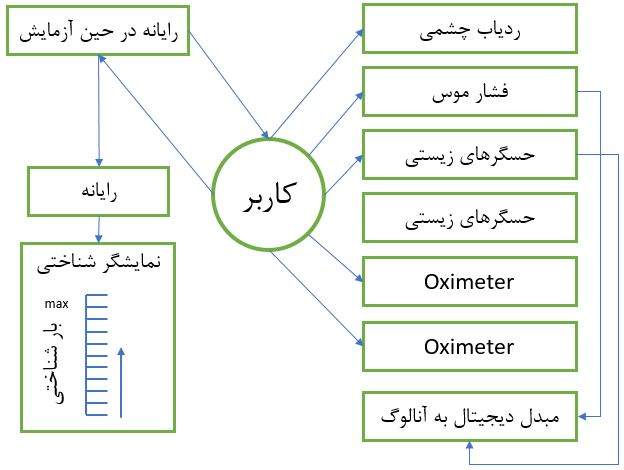
\includegraphics[width=0.7\linewidth]{figures/ikehara2005}
	\caption[نمونه‌ای از سیستم حسگرهای فیزیولوژیکی]{سیستم ها و جریان اطلاعات در آزمایش MTF}
	\label{fig:ikehara2005}
\end{figure}
چِن و همکاران
\cite{Chen2011}
با ۱۲ بسکتبالیست غیرحرفه‌ی ۱۹ تا ۳۶ سال که مبلغی نیز به آن‌ها پرداخت شده بود سعی در اندازه گیری بار شناختی آنها با ۸ داده چشمی داشتند. آزمایش آنها یک برنامه کامپیوتری یادگیری بود، که به کاربر استراتژی بازی را با مشخص کردن مدافعان و مهاجم‌ها و مکانشان نسبت به توپ آموزش می‌داد.
هشت متغیر وابسته برای اندازه‌گیری فشار ذهنی استفاده شدند. شامل: تاخیر در پلک زدن، نرخ پلک زدن، میانگین اندازه مردمک چشم بین ثانیه دوم و انتهای بازی، انحراف معیار در ثانیه چهارم، زمان تثبیت، نرخ تثبیت،‌ اندازه پرش و سرعت پرش چشم.
با توجه به تفاوت در بازه‌ی داده‌های کاربران آنها با رابطه
\eqref{eq:normalize}
در یک بازه قرار می‌دادند.
\begin{equation}\label{eq:normalize}
V_{cal} = \dfrac{V_{raw}-V_{min}}{V_{max}-V_{min}}
\end{equation} 
در پایان مشاهده شد معیارهای مختلف چشمی مثل داده‌هایی که از پلک زدن، حرکت‌های چشم و اندازه مردمک بدست می‌آیند تفاوت روشنی در دو فشار ذهنی کم و زیاد با یک آموزش رایانه‌ای نشان می‌دهد. آنها این معیارها را را قدم اولیه‌ای برای اندازه گیری فشارذهنی به صورت هم زمان معرفی نمودند.
\\

روتستین و همکاران
\cite{ozeri2020relationship}
با برسی ۱۹ کودک بین ۸ تا ۱۲ ساله با زبان مادری انگلیسی که مشکل‌های خواندن داشتند در آزمایشی همراه والدین‌شان به بیمارستان آمده و به آن‌ها دو دسته متن نمایش داده شد، دسته اول جمله‌هایی که پیام و مفهوم خاصی دنبال می‌کنند و دسته دوم جمله‌هایی بدون مفهوم و معنی. به آنها گفته می‌شد تا جایی که امکان دارد درست و سریع پاسخ دهند. با بررسی قطر مردمک چشم و تثبیت توانستند رابطه‌ای میان بارشناختی و داده های چشمی پیدا کنند.
